\documentclass[tikz,border=8pt]{standalone}
\usetikzlibrary{arrows.meta,positioning,shapes.geometric}
\begin{document}
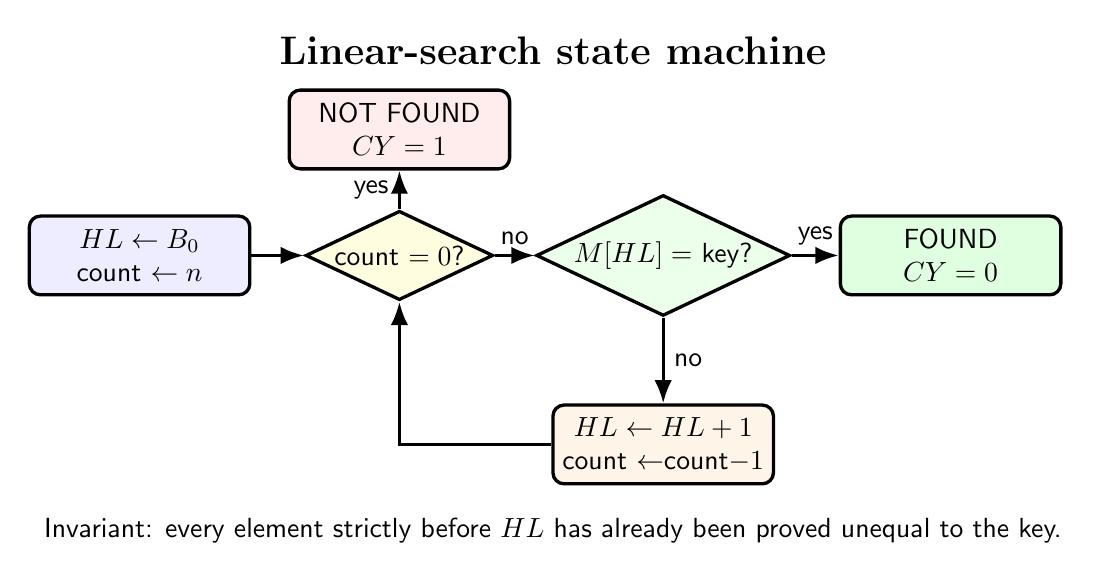
\begin{tikzpicture}[font=\sffamily,>=Latex,
 state/.style={draw,very thick,rounded corners,minimum width=2.8cm,minimum height=1cm,align=center},
 test/.style={draw,very thick,diamond,aspect=2.1,align=center,inner sep=1pt}]
\node[font=\Large\bfseries] at (6.6,6.25) {Linear-search state machine};
\node[state,fill=blue!7] (start) at (1.35,3.65) {$HL\leftarrow B_0$\\count $\leftarrow n$};
\node[test,fill=yellow!12] (empty) at (4.65,3.65) {count $=0$?};
\node[test,fill=green!8] (cmp) at (8.0,3.65) {$M[HL]=$ key?};
\node[state,fill=red!7] (miss) at (4.65,5.25) {NOT FOUND\\$CY=1$};
\node[state,fill=green!12] (found) at (11.65,3.65) {FOUND\\$CY=0$};
\node[state,fill=orange!9] (step) at (8.0,1.25) {$HL\leftarrow HL+1$\\count $\leftarrow$count$-1$};
\draw[very thick,->] (start)--(empty);
\draw[very thick,->] (empty)-- node[above] {no} (cmp);
\draw[very thick,->] (empty)-- node[left] {yes} (miss);
\draw[very thick,->] (cmp)-- node[above] {yes} (found);
\draw[very thick,->] (cmp)-- node[right] {no} (step);
\draw[very thick,->] (step.west)-|(empty.south);
\node at (6.6,.15) {Invariant: every element strictly before $HL$ has already been proved unequal to the key.};
\end{tikzpicture}
\end{document}
